%   % !TEX root = ../../VIII,3_Rahmen-TeX_8-1.tex
%   ####
%
%   Band VIII, 3 N.~??A14 // Akustik, Elastizität, Festigkeit
%   Signatur/Tex-Datei: LH_35_09_15_001,022
%   RK-Nr. 41157
%   Überschrift: [De tensione et restitutione]
%   Datierung: [Sommer 1678 bis Winter 1680/1681 (?)]
%   WZ: LEd-Wz 803002 = RK-WZ: 138 (Achtblättrige Rosette auf CS)
%.  SZ: \leibvdash (insgesamt eins)
%.  Bilddateien (PDF): LH_35_09_15_001,022_d1; LH_35_09_15_001,022_d2; LH_35_09_15_001,022_d3; LH_35_09_15_001,022_d4; LH_35_09_15_001,022_d5; LH_35_09_15_001,022_d6 (insgesamt: sechs)
%
%
\selectlanguage{ngerman}%
\frenchspacing%
%
\begin{ledgroupsized}[r]{120mm}
\footnotesize
\pstart
\noindent
\textbf{Überlieferung:}
\pend
\end{ledgroupsized}
\begin{ledgroupsized}[r]{114mm}
\footnotesize
\pstart \parindent -6mm
\makebox[6mm][l]{\textit{L}}%
Aufzeichnung: LH~XXXV~9,~15 Bl.~1, 22.
Zwei Blatt~4\textsuperscript{o},
die ursprünglich einen \mbox{Bogen} bildeten;
zusammenhängende Hälften eines Wasserzeichens auf Bl.~1 und Bl.~22.
Vier Seiten, zumeist einspaltig beschrieben;
Textfolge gemäß Blattzählung;
gesamter Text (Diagramme, Rechnungen und Randbemerkungen mit eingeschlossen) gestrichen.
% Auf der rechten Spalte von Bl.~22~v\textsuperscript{o} finden sich,
% ebenfalls gestrichen, Rechnungen und Diagramme,
% die keinen unmittelbaren Zusammenhang mit dem Text aufweisen.
Bl.~1 und Bl.~22 waren ursprünglich mit LH~XXXV~11,~14 Bl.~18,
einem der Textträger von \textit{LSB} VI,~4 N.~267,\cite{01339} verbunden.
\pend
\end{ledgroupsized}
%
%
\vspace{5mm}
\begin{ledgroup}
\footnotesize
\pstart
\noindent
\textbf{Datierungsgründe:}\label{LH_35_09_15_001,022_Datierung}
In der vorliegenden Aufzeichnung N.~7 erörtert Leibniz im Rahmen seiner Elastizitätslehre vornehmlich den Begriff der Spannung (\textit{tensio}) als Ursache elastischer Wiederherstellung (\textit{restitutio}).
Als ausschlaggebend für die Datierung erweist sich der Überlieferungszusammenhang mit dem Text \textit{Definitiones cogitationesque metaphysicae} (\textit{LSB} VI,~4 N.~267\cite{01339}),
mit dem die Aufzeichnung N.~7 ursprünglich einen einheitlichen Folio-Bogen bildete; vom Duktus her könnte N.~7 sogar als Ableger der umfangreicheren \textit{Definitiones cogitationesque metaphysicae} entstanden sein.
Das für die frühe Hannoveraner Zeit gewöhnliche Wasserzeichen im Träger von N.~7 ist im Nachlass für den Zeitraum vom Sommer 1678 bis zum Winter 1680/1681 belegt.
Aus inhaltlichen Gründen kann man aber ausschließen, dass die \textit{Definitiones cogitationesque metaphysicae} vor dem Frühjahr 1679 entstanden (vgl. VI,~4, S.~1393.18\textendash21).
Eine Entstehungszeit zwischen Frühjahr 1679 und Winter 1680/1681 ist somit grundsätzlich auch für N.~7 anzunehmen.
\pend%
\pstart%
Es gilt allerdings zu bemerken, dass der Aufzeichnung N.~7 offenbar eine kritische Auseinandersetzung mit H.~\textsc{Fabri}, \textit{Physica}, tract.~I, lib. II: \textit{De compresso et tenso} (Bd.~I, Lyon 1669, S.~42\,ff.) zugrunde liegt.
Mit dieser in einer Randbemerkung (S.~\pageref{LH_35_09_15_022r_rndbmrkng_czjt}) ausdrücklich erwähnten Quelle hängen weitere, thematisch verwandte und in diesem Band edierte Texte zusammen, die auf Dezember 1680 oder Anfang 1681 datierbar sind: etwa N.~8 (\textit{Tentaminum de chordarum tensione schedae}), N.~9 (\textit{Motuum restitutionis regula}) und N.~10 (\textit{De chordarum tensione}).
Dieser Zusammenhang lässt die Vermutung zu, dass die Entstehungszeit der Aufzeichnung N.~7 (sowie der \textit{Definitiones cogitationesque metaphysicae}\cite{01339}) ebenfalls auf den Winter 1680/1681 eingeschränkt werden kann.
\pend
\end{ledgroup}
%
%
%
\selectlanguage{latin}%
\frenchspacing%
%
%
\vspace{8mm}
\count\Bfootins=1100
\count\Afootins=1100
\count\Cfootins=1100
\pstart%
\footnotesize%
\noindent%
%
{\normalsize{\lbrack1~r\textsuperscript{o}\rbrack}}% % Blatt 1r
%
\textso{ Compressio }\protect\index{Sachverzeichnis}{compressio}%
nihil aliud est quam expressio\protect\index{Sachverzeichnis}{expressio materiae}
\edtext{materiae tenuioris,\protect\index{Sachverzeichnis}{materia tenuis}}{%
\lemma{materiae}\Bfootnote{%
\textit{(1)}~subtilioris,\protect\index{Sachverzeichnis}{materia subtilis}
\textit{(2)}~tenuioris,%
~\textit{L}}}
quae cum motu quodam suo\protect\index{Sachverzeichnis}{motus materiae}
denuo poros\protect\index{Sachverzeichnis}{porus} subeat,
remque compressam\protect\index{Sachverzeichnis}{res compressa}
iterum\textso{ dilatet,}
hinc oritur\textso{ restitutio.}\protect\index{Sachverzeichnis}{restitutio}
Exemplum\protect\index{Sachverzeichnis}{exemplum} habemus in
\edtext{massa compacta\protect\index{Sachverzeichnis}{massa compacta} ex}{%
\lemma{massa}\Bfootnote{%
\hspace{-0,5mm}compacta ex \textit{erg.~L}}}
charta aliqua bibula,\protect\index{Sachverzeichnis}{charta bibula} vel simili corpore,
cui si humorem\protect\index{Sachverzeichnis}{humor} expresseris,
\edtext{ipsumque corpus siccari curaveris,}{%
\lemma{ipsumque}\Bfootnote{%
\textit{(1)}~siccari \textbar~curaveris \textit{streicht Hrsg.}~\textbar\
\textit{(2)}~corpus siccari curaveris,%
~\textit{L}}}
si
\edtext{denuo aquam\protect\index{Sachverzeichnis}{aqua}}{%
\lemma{denuo}\Bfootnote{%
\textit{(1)}~aquae
\textit{(2)}~aquam%
~\textit{L}}}
immittas,
videbis
\edtext{\lbrack id\rbrack}{%
\lemma{id}\Bfootnote{\textit{erg. Hrsg.}}}
iterum inflari.
Quod si in media aqua manu comprimas,
videbis mox sponte\lbrack,\rbrack\
id est aquae subingredientis nisu\lbrack,\rbrack\protect\index{Sachverzeichnis}{nisus aquae subingredientis}
iterum inflari.
\pend%
%
\pstart%
\footnotesize%
Omnia corpora compressionis et restitutionis capacia sunt,%
\protect\index{Sachverzeichnis}{corpus capax compressionis}%
\protect\index{Sachverzeichnis}{corpus capax restitutionis}
alioqui leges motus\protect\index{Sachverzeichnis}{lex motus}
(\protect\vphantom)%
\edtext{quas ex metaphysicis principiis\protect\index{Sachverzeichnis}{principium metaphysicum}
demonstravimus}{%
\lemma{quas \lbrack...\rbrack\ demonstravimus}\Cfootnote{%
Wohl Anspielung auf das Konzept \textit{Principia mechanica ex metaphysicis dependere} (\textit{LSB} VI,~4 N.~362\cite{01338}), das auf Sommer 1678 bis Winter 1680/81\,(?) datiert ist.}}%
\protect\vphantom()
in natura\protect\index{Sachverzeichnis}{natura} servari non possent.
\pend%
%
\pstart%
\footnotesize%
\textso{Compressio }\protect\index{Sachverzeichnis}{compressio}%
est redactio\protect\index{Sachverzeichnis}{redactio materiae}
ejusdem materiae sensibilis\protect\index{Sachverzeichnis}{materia sensiblilis}
in minus spatium,%
\textso{ Distensio }\protect\index{Sachverzeichnis}{distensio}%
\edtext{vel\textso{ diductio }\protect\index{Sachverzeichnis}{diductio}}{%
\lemma{vel}\Bfootnote{%
\hspace{-0,5mm}\textso{diductio} \textit{erg.~L}}}%
ad \edtext{majus.
Utramque communi nomine\protect\index{Sachverzeichnis}{nomen commune}%
\textso{ Tensionem }\protect\index{Sachverzeichnis}{tensio}vocabo.
Nam arcus tensus\protect\index{Sachverzeichnis}{arcus tensus}
partim compressus,\protect\index{Sachverzeichnis}{arcus compressus}
partim diductus\protect\index{Sachverzeichnis}{arcus diductus} est,
illud a concavo, hoc a convexo.
\newline%
\indent%
Omnis tensio\protect\index{Sachverzeichnis}{tensio}}{%
\lemma{majus.}\Bfootnote{%
\hspace{-0,5mm}\textbar~%
\textit{(1)}~Uterque
\textit{(2)}~Utramque communi \lbrack...\rbrack\ a convexo. \textit{erg.}~%
\textbar\ Omnis 
\textit{(1)}~compressio et
\textit{(2)}~tensio%
~\textit{L}}}
cum restituendi conatu\protect\index{Sachverzeichnis}{conatus restituendi} conjuncta est.
Est observatio\protect\index{Sachverzeichnis}{observatio}
potius quam theorema.\protect\index{Sachverzeichnis}{theorema}
Unde colligitur\lbrack:\rbrack\
quandocunque sola materia insensibilis\protect\index{Sachverzeichnis}{materia insensibilis}
\edtext{exprimitur\protect\index{Sachverzeichnis}{expressio materiae}
ut in compressione\protect\index{Sachverzeichnis}{compressio}
vel sugitur\protect\index{Sachverzeichnis}{suctio materiae}
ut in diductione,\protect\index{Sachverzeichnis}{diductio}
eam redire conari ad statum priorem.\protect\index{Sachverzeichnis}{status prior}}{%
\lemma{exprimitur}\Bfootnote{%
\textit{(1)}~fieri te
\textit{(2)}~ut in \lbrack...\rbrack\ ut in 
\textit{(a)}~tensione
\textit{(b)}~diductione, eam \lbrack...\rbrack\ statum priorem.%
~\textit{L}}}
Adeoque omnem materiam insensibilem\protect\index{Sachverzeichnis}{materia insensibilis}
in motu esse.\protect\index{Sachverzeichnis}{motus materiae}
\pend%
%
\pstart%
\footnotesize%
Motus restitutionis\protect\index{Sachverzeichnis}{motus restitutionis}
est acceleratus,\protect\index{Sachverzeichnis}{motus acceleratus}
nam praeter conceptum jam
\edtext{impetum\protect\index{Sachverzeichnis}{impetus conceptus} ex}{%
\lemma{impetum}\Bfootnote{%
\textit{(1)}~in
\textit{(2)}~ex%
~\textit{L}}}
jam facta restitutione,\protect\index{Sachverzeichnis}{restitutio}
novus\protect\index{Sachverzeichnis}{impetus novus} durante adhuc motu
imprimitur,\protect\index{Sachverzeichnis}{impetus impressus}
durat enim status violentus,\protect\index{Sachverzeichnis}{status violentus}
adeoque conatus\protect\index{Sachverzeichnis}{conatus restitutionis}
\edtext{restitutionis.
%
{\normalsize{\lbrack1~v\textsuperscript{o}\rbrack}} % Blatt 1v
%
\newline%
\indent%
Quod chorda\protect\index{Sachverzeichnis}{chorda}
sagittam\protect\index{Sachverzeichnis}{sagitta}
non ante projicit quam ubi}{%
\lemma{restitutionis.}\Bfootnote{%
\textit{(1)}~Corpus quod acceleratur aliud quod ante se propellit
\lbrack1~v\textsuperscript{o}\rbrack\
\textit{(2)}~Quod chorda sagittam non ante
\textit{(a)}~ejaculari potest, quam ubi
\textit{(b)}~projicit quam ubi%
~\textit{L}}}
ipsa progredi non potest;
hujus rei causa\protect\index{Sachverzeichnis}{causa}
non est sola acceleratio,\protect\index{Sachverzeichnis}{acceleratio}
neque etiam quod sagitta non est
\edtext{notabiliter levior quam chorda,}{%
\lemma{notabiliter}\Bfootnote{%
\textit{(1)}~chorda
\textit{(2)}~levior quam chorda,%
~\textit{L}}}
sed quod chorda\protect\index{Sachverzeichnis}{chorda}
sagittam\protect\index{Sachverzeichnis}{sagitta} inde a quiete\protect\index{Sachverzeichnis}{quies} secum duxit.
Ita enim corpus magnum\protect\index{Sachverzeichnis}{corpus magnum} non potest
\edtext{se}{%
\lemma{se}\Bfootnote{\textit{erg.~L}}}
celerius impellere minus,
quia nulla fit\protect\index{Sachverzeichnis}{percussio}
percussio.\edlabel{LH_35_09_15_001v_pervir-1}%
\edtext{}{\lemma{\textit{Am Satzende, zwischenzeilig:}}\Afootnote{%
{\footnotesize{In hoc lapsus.}}\protect\index{Sachverzeichnis}{lapsus}
\textit{Hierauf folgt ein Zuweisungszeichen, das sich nicht zuordnen lässt.}}}
\edtext{}{%
{\xxref{LH_35_09_15_001v_pervir-1}{LH_35_09_15_001v_pervir-2}}%
{\lemma{percussio.}\Bfootnote{%
\textit{(1)}~Tantus est conatus resti
\textit{(2)}~Vis quae tetendit aut compressit,
\textit{(a)}~$\langle$vis$\rangle$
\textit{(b)}~spatium
\textit{(c)}~et vis restituendi\protect\index{Sachverzeichnis}{vis restituendi}
\textit{(3)}~Vires tendentes
\textit{(a)}~aut comprimentes,\protect\index{Sachverzeichnis}{vis comprimens} itemque conatus restituendi
\textit{(b)}~, vel quod \lbrack...\rbrack\ conatus restituendi,%
~\textit{L}}}}
\pend%
  \vspace*{1,0em}%
%
%
  \centerline{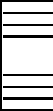
\includegraphics[width=0.070\textwidth]{gesamttex/edit_VIII,3/images/LH_35_09_15_001,022_d1.pdf}}%
  \vspace*{0.5em}
  \centerline{\lbrack\textit{Fig.~1}\rbrack}%
%
%
  \newpage%  Rein vorläufig !!!!
%  \vspace*{1.0em}%
\pstart%
\footnotesize%
Vires tendentes,%
\protect\index{Sachverzeichnis}{vis tendens} % \lbrack,\rbrack\
vel quod idem est conatus restituendi,%
\protect\index{Sachverzeichnis}{conatus restituendi}\edlabel{LH_35_09_15_001v_pervir-2} % \lbrack,\rbrack\
sunt inter se ut rationes spatiorum praeternaturalium\protect\index{Sachverzeichnis}{spatium praeternaturale}
\edtext{naturalibus accedentium}{%
\lemma{naturalibus}\Bfootnote{%
\hspace{-0,5mm}accedentium
\textit{erg.~L}}}
ad spatia naturalia.\protect\index{Sachverzeichnis}{spatium naturale}
Sint
\edtext{vires tendentes\protect\index{Sachverzeichnis}{vis tendens}}{%
\lemma{vires}\Bfootnote{%
\textit{(1)}~turbantes\protect\index{Sachverzeichnis}{vis turbans}
\textit{(2)}~tendentes%
~\textit{L}}}
\textit{T.} \textit{t.}
Restituentes\protect\index{Sachverzeichnis}{vis restituens} \textit{R.} \textit{r.}
Spatia praeternaturalia\protect\index{Sachverzeichnis}{spatium praeternaturale} \textit{P.} \textit{p.}
Naturalia\protect\index{Sachverzeichnis}{spatium naturale} \textit{N.} \textit{n.}
Erit \textit{T} ad \textit{t},
vel quod idem est \textit{R} ad \textit{r},
ut % \protect\rule[0pt]{0mm}{12pt}
$\displaystyle\frac{P}{N}$ ad
\edtext{$\displaystyle\frac{N}{n}.$
Nam tanta est vis quanta turbatio,\protect\index{Sachverzeichnis}{turbatio}
vel si mavis quanta % 
materiae tenuis\protect\index{Sachverzeichnis}{materia tenuis}
rediturientis\protect\index{Sachverzeichnis}{materia redituriens}
expressio\protect\index{Sachverzeichnis}{expressio materiae}
vel insuctio.\protect\index{Sachverzeichnis}{insuctio materiae}}{% \protect\rule[0pt]{0mm}{8pt}
\lemma{$\displaystyle\frac{N}{n}.$}\Bfootnote{%
\textit{(1)}~Si fingamus corpus quod jam intus est non posse comprimi,\protect\index{Sachverzeichnis}{corpus incomprimibile} res manifesta. Jam etsi comprimi posset\protect\index{Sachverzeichnis}{corpus comprimibile}
\textit{(a)}~tantu
\textit{(b)}~non ideo vis major minorve requiretur
\textit{(aa)}~ad
\textit{(bb)}~tantum enim materiae tenuis quae ex uno exprimenda fuisset, expressa fuisset ex duobus.
\textit{(2)}~Nam
\textit{(3)}~Breve 
\textit{(4)}~Brevius:
\textit{(5)}~N
\textit{(6)}~Nam tanta \lbrack...\rbrack\ vel insuctio.%
~\textit{L}}}
%
\edtext{Idem alibi rigorosius demonstravi.}{%
\lemma{Idem \lbrack...\rbrack\ demonstravi}\Cfootnote{%
Vermutlich Anspielung auf G.\,W. \textsc{Leibniz}, \textit{Hypothesis physica nova}, Mainz 1671, § 27 (\textit{LSB}
VI,~2 N.~40, S.~234\,f.).\cite{00256}}}
\pend%
%  \newpage
  \vspace{2.0em}%
%
%
  \centerline{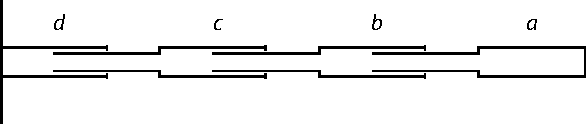
\includegraphics[width=0.56\textwidth]{gesamttex/edit_VIII,3/images/LH_35_09_15_001,022_d2.pdf}}%
  \vspace{-0.5em}
  \centerline{\lbrack\textit{Fig.~2}\rbrack}%
  \label{LH_35_09_15_001v_fig.2}
%
%
  \vspace{2.0em}%
\pstart%
\footnotesize%
Corporis\edlabel{LH_35_09_15_001v_gleichSpann_irls-1} uniformis tensi%
\protect\index{Sachverzeichnis}{corpus uniforme}\protect\index{Sachverzeichnis}{corpus tensum}
quaelibet pars aequaliter tensa est,\protect\index{Sachverzeichnis}{pars aequaliter tensa}
si nulla gravitatis\protect\index{Sachverzeichnis}{gravitas} partium ratio habeatur.
Sit
%
\edtext{embolus\protect\index{Sachverzeichnis}{embolus} corporis \textit{a}}{%
\lemma{embolus corporis \textit{a}}\Cfootnote{%
Siehe das Diagramm \lbrack\textit{Fig.~2}\rbrack.}}
%
in capacitate corporis\protect\index{Sachverzeichnis}{capacitas corporis} \textit{b},
embolus\protect\index{Sachverzeichnis}{embolus} corporis \textit{b}
in capacitate ipsius \textit{c},
%
{\normalsize{\lbrack22~r\textsuperscript{o}\rbrack}} % Blatt 22r
%
et corporis \textit{c} in capacitate\protect\index{Sachverzeichnis}{capacitas corporis} ipsius \textit{d}
eodem ubique modo,
nec educi ullus eorum possit sine
\edtext{vi;\protect\index{Sachverzeichnis}{vis tendens}
ob tensionem\protect\index{Sachverzeichnis}{tensio} scilicet}{%
\lemma{vi;}\Bfootnote{%
\textit{(1)}~si quis jam
\textit{(2)}~ob tensionem scilicet%
~\textit{L}}}
quae inde sequitur.
\edtext{Ponamus educi corpus \textit{a}.}{%
\lemma{Ponamus}\Bfootnote{%
\textit{(1)}~adduci
\textit{(2)}~educi
\textbar~primum \textit{streicht}~%
\textbar\ corpus \textit{a}.%
~\textit{L}}}
Cumque eodem omnia modo connexa sint,
nec unum sine altero moveri possit
nisi supposita jam aliqua tensione,\protect\index{Sachverzeichnis}{tensio}
nec ratio sit cur ullum prae altero moveatur,
tenduntur onmia aequaliter.
\edtext{A gravitate\protect\index{Sachverzeichnis}{gravitas} autem
seu mole corporis\protect\index{Sachverzeichnis}{moles corporis}
abstrahendus est animus,\protect\index{Sachverzeichnis}{animus}
alioqui enim facilius movebitur minus quam majus.
Unde causa rupturae\protect\index{Sachverzeichnis}{causa rupturae}
in loco uno potius quam alio duci potest,
etiam in diducendo homogeneo.%
\edlabel{LH_35_09_15_001v_gleichSpann_irls-2}%
\protect\index{Sachverzeichnis}{corpus diducendum}}{%
\lemma{A}\Bfootnote{%
\hspace{-0,5mm}gravitate \lbrack...\rbrack\ facilius movebitur
\textit{(1)}~majus
\textit{(2)}~minus quam \lbrack...\rbrack\ etiam in
\textbar~in \textit{streicht Hrsg.}~%
\textbar\ diducendo homogeneo.
\textit{erg.~L}}}
\pend%
%  \newpage% Rein vorläufig !!!!
  \vspace{2.4em}%
%
%
  \centerline{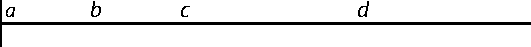
\includegraphics[width=0.54\textwidth]{gesamttex/edit_VIII,3/images/LH_35_09_15_001,022_d3.pdf}}%
  \vspace{0.5em}
  \centerline{\lbrack\textit{Fig.~3}\rbrack}%
    \label{LH_35_09_15_001v_fig.3}
%
%
  \newpage% Rein vorläufig !!!!
%  \vspace*{1.0em}%
\pstart%
\footnotesize%
Hinc
\edtext{}{%
{\xxref{LH_35_09_15_022r_klnbchst-1}{LH_35_09_15_022r_klnbchst-2}}%
{\lemma{\textit{AB} \lbrack...\rbrack\ \textit{AC}}\Cfootnote{%
Gemeint sind Strecken der Saite \textit{ABC} nach dem Diagramm \lbrack\textit{Fig.~3}\rbrack\ auf S.~\pageref{LH_35_09_15_001v_fig.3},
wo sie aber durch Kleinbuchstaben bezeichnet werden.}}}%
\edtext{sit \textit{AB}\edlabel{LH_35_09_15_022r_klnbchst-1} aequ.}{%
\lemma{sit}\Bfootnote{%
\textit{(1)}~\textit{ab} aeq
\textit{(2)}~\textit{AB} aequ.%
~\textit{L}}}
\textit{BC}, et \textit{CD} aequ. \textit{AC}.\edlabel{LH_35_09_15_022r_klnbchst-2}
Si
\edtext{chorda\protect\index{Sachverzeichnis}{chorda tensa} \textit{ABC} tendatur,
manente}{%
\lemma{chorda}\Bfootnote{%
\textit{(1)}~\textit{abc}
\textit{(2)}~\textit{ABC}
\textit{(a)}~ten
\textit{(b)}~diducatur, ma
\textit{(c)}~tendatur, manente%
~\textit{L}}}
puncto \textit{A}
\edtext{immobili,\protect\index{Sachverzeichnis}{punctum immobile}
et punctum \textit{C} perveniat}{%
\lemma{immobili,}\Bfootnote{%
\hspace{-0,5mm}et
\textit{(1)}~\textit{b} perven
\textit{(2)}~\textit{C}
\textit{(3)}~punctum \textit{C} perveniat%
~\textit{L}}}
in \textit{D},
tunc punctum \textit{B} perveniet in
\edtext{\lbrack\textit{C}\rbrack.}{%
\lemma{\textit{D}}\Bfootnote{%
\textit{L~ändert Hrsg.}}}
Ita enim
\edtext{partes \textit{AB} et \textit{BC}}{%
\lemma{partes}\Bfootnote{%
\textit{(1)}~\textit{ab}
\textit{(2)}~\textit{AB} et
\textit{(a)}~\textit{CD}
\textit{(b)}~\textit{BC}%
~\textit{L}}}
erunt aequaliter tensae\protect\index{Sachverzeichnis}{pars aequaliter tensa}\lbrack,\rbrack\
\edtext{quia pars \textit{AB} occupat locum \textit{AC},}{%
\lemma{quia}\Bfootnote{%
\hspace{-0,5mm}\textbar~pars \textit{erg.}~%
\textbar\ \textit{AB} occupat
\textbar~locum \textit{erg.}~%
\textbar\ \textit{AC},
\textit{L}}}
et pars
\edtext{ei aequalis}{%
\lemma{ei}\Bfootnote{%
\hspace{-0,5mm}aequalis
\textit{erg.~L}}}
\textit{BC} locum \textit{CD} priori loco aequalem.
\pend%
% \newpage%
%
\pstart%
\footnotesize%
\edtext{Hinc sequitur spatia\protect\index{Sachverzeichnis}{spatium percursum}
quae inter tensionem\protect\index{Sachverzeichnis}{tensio chordae}
puncta chordae\protect\index{Sachverzeichnis}{punctum chordae} percurrunt
esse distantiis a puncto immobili\protect\index{Sachverzeichnis}{punctum immobile} proportionalia.
Et quia etiam omnia simul restituuntur,
et durante restitutione\protect\index{Sachverzeichnis}{restitutio chordae}
\edtext{semper eundem gradum tensionis\protect\index{Sachverzeichnis}{gradus tensionis} retinent}{%
\lemma{semper}\Bfootnote{%
\textit{(1)}~eodem modo tensa
\textit{(2)}~eundem gradum tensionis retinent%
~\textit{L}}}
usque ad plenam restitutionem,\protect\index{Sachverzeichnis}{restitutio plena}
hinc eadem esse
\edtext{debet ratio celeritatum\protect\index{Sachverzeichnis}{ratio celeritatum}
in restitutione\protect\index{Sachverzeichnis}{restitutio chordae} quae}{%
\lemma{debet}\Bfootnote{%
\textit{(1)}~celeritas in restitutione quae
\textit{(2)}~ratio celeritatum in restitutione quae%
~\textit{L}}}
est in tensione\protect\index{Sachverzeichnis}{tensio chordae}%
\protect\label{LH_35_09_15_022r_rndbmrkng_czjt}%
%%%%
%%%%    ANFANG DER MARGINALIE
}{\lemma{\textit{Auf der rechten Spalte:}}\Afootnote{%
{\footnotesize%
Imo in eo erratum,\protect\index{Sachverzeichnis}{erratum}
nam sive alterutrum extremum sit immobile,
sive utrinque trahatur,
idem est,\protect\index{Sachverzeichnis}{extremum chordae}
tantum enim duo extrema a se invicem discedunt,
chorda\protect\index{Sachverzeichnis}{chorda tensa} enim
vi tensionis\protect\index{Sachverzeichnis}{vis tensionis}
suae\protect\index{Sachverzeichnis}{tensio chordae}
unum continuum\protect\index{Sachverzeichnis}{unum continuum} est,
adeoque%
\textsuperscript{[a]}
potius mediorum punctorum tardior erit motus%
\protect\index{Sachverzeichnis}{motus puncti medii}\lbrack,\rbrack\
in quo et%
\textsuperscript{[b]}
erratum est ab Honorato Fabry.\protect\index{Namensregister}{\textso{Fabri}, Honoré 1607\textendash1688}%
\textsuperscript{[c]}
Re recte expensa%
\textsuperscript{[d]}
eo redit quaestio\protect\index{Sachverzeichnis}{quaestio} an corpus faclius moveatur quam tendatur%
\textsuperscript{[e]}
sive an facilius moveatur majus quam tendatur minus.
Puto totum corpus simul recipere conatum\protect\index{Sachverzeichnis}{conatus} primo momento,
quia ab initio nulla%
\textsuperscript{[f]}
fit tensio,\protect\index{Sachverzeichnis}{tensio corporis}
sed initio statim est continui motus.\protect\index{Sachverzeichnis}{motus continui}%
\newline%
\newline%
% \\%
%%%%
\textsuperscript{[a]}~%
adeoque
\textit{(1)}~in medio
\textit{(2)}~potius mediorum punctorum%
~\textit{L}
\quad
%%%%
\textsuperscript{[b]}~%
et
\textit{erg.~L}
\quad
%%%%
\textsuperscript{[c]}~%
erratum \lbrack...\rbrack\ Fabry:
Siehe H.\,\textsc{Fabri}, \textit{Physica}, tract. I, lib. II, prop. LXI (Bd.~I, Lyon 1669, S.~63).\cite{00044}
Leibniz hat die Stelle sowohl in seinem Handexemplar angestrichen wie auch exzerpiert; vgl. \textit{LSB} VI,~2 N.~39\textsubscript{3}, S.~212.14\textendash15;\cite{01234} VIII,~2 N.~55, S.~471.7\textendash9.\cite{01120}
\quad
%%%%
\textsuperscript{[d]}~%
expensa
\textit{(1)}~ab
\textit{(2)}~eo%
~\textit{L}
\quad
%%%%
\textsuperscript{[e]}~%
tendatur
\textit{(1)}~. Sed jam tamen video hoc loco necessario
\textit{(2)}~sive an \lbrack...\rbrack\ tendatur minus.
\textit{(a)}~Si totum corpus simul recipit conat
\textit{(b)}~Et
\textit{(c)}~Puto totum \lbrack...\rbrack\ recipere conatum%
~\textit{L}
\quad
%%%%
\textsuperscript{[f]}~%
nulla
\textit{(1)}~est
\textit{(2)}~fit%
~\textit{L}}}}%
%%%%    ENDE DER MARGINALIE
%%%%
\edtext{.%
\newline%
\indent%
Cum corpus sibi relinquitur,}{%
\lemma{tensione.}\Bfootnote{%
\textit{(1)}~Durante motu restitutionis spontaneo\protect\index{Sachverzeichnis}{motus restitutionis}
\textit{(2)}~Cum corpus sibi relinquitur,%
~\textit{L}}}
causa restituens\protect\index{Sachverzeichnis}{causa restituens}
omnibus partibus aequalem vim
\edtext{imprimit,\protect\index{Sachverzeichnis}{vis impressa}
quare tota vis impressa}{%
\lemma{imprimit,}\Bfootnote{%
\textit{(1)}~itaque quo minus est corpus
\textit{(2)}~quare tota vis impressa%
~\textit{L}}}
aequaliter distribuitur in omnes partes.\protect\index{Sachverzeichnis}{vis aequaliter distributa}
Hinc quo pauciores partes\lbrack,\rbrack\
hoc in singulis major impetus.\protect\index{Sachverzeichnis}{impetus restitutionis}
Sint ergo mille corpora ex tubis\protect\index{Sachverzeichnis}{tubum}
%
{\normalsize{\lbrack22~v\textsuperscript{o}\rbrack}} % Blatt 22v
%
embolisque\protect\index{Sachverzeichnis}{embolus} composita ut in
\edtext{figura\protect\index{Sachverzeichnis}{figura} superiore}{%
\lemma{figura superiore}\Cfootnote{%
Das Diagramm \lbrack\textit{Fig.~2}\rbrack\ auf S.~\pageref{LH_35_09_15_001v_fig.2}.}}%
\lbrack,\rbrack\
\edtext{diducantur ad longitudinem\protect\index{Sachverzeichnis}{longitudo corporis diducti} duplam,}{%
\lemma{diducantur}\Bfootnote{%
\hspace{-0,5mm}ad
\textit{(1)}~spatium
\textit{(a)}~decuplo majus
\textit{(b)}~duplo majus
\textit{(2)}~longitudinem
\textit{(a)}~duplo majorem
\textit{(b)}~duplam,%
~\textit{L}}}
sint alia bis mille,
quae diducantur etiam ad longitudinem duplam suae prioris.
Cum corpora ubique sint aequalia,
et diductio\protect\index{Sachverzeichnis}{diductio}
\edtext{etiam,
sed corpora diducenda\protect\index{Sachverzeichnis}{corpus diducendum} sint duplo plura,
patet,}{%
\lemma{etiam,}\Bfootnote{%
\textit{(1)}~patet
\textit{(2)}~sed corpora \lbrack...\rbrack\ plura, patet,%
~\textit{L}}}
duplo majori vi\protect\index{Sachverzeichnis}{vis deductionis} opus esse in posteriore
\edtext{casu.
Idem est in compressione.\protect\index{Sachverzeichnis}{compressio}
Itaque si corpora eadem ratione tensa sint,\protect\index{Sachverzeichnis}{corpus tensum}
id est ut spatium sit in eadem ratione multiplicatum vel submultiplicatum,
vires tendentes\protect\index{Sachverzeichnis}{vis tendens} erunt}{%
\lemma{casu.}\Bfootnote{%
\textit{(1)}~Itaque vires erunt
\textit{(2)}~Id enim
\textit{(3)}~Idem est in compressione
\textit{(4)}~Idem est \lbrack...\rbrack\ sit in eadem
\textit{(a)}~ratione auctum vel diminutum,
\textit{(b)}~\textbar~ratione \textit{erg.}~\textbar\ multiplicatum vel \lbrack...\rbrack\ tendentes erunt%
~\textit{L}}}
ut corpora ejusdem materiae.%
\protect\index{Sachverzeichnis}{magnitudo corporis}\protect\index{Sachverzeichnis}{materia corporis}
Idemque etiam ex eo
\edtext{demonstratur, si}{%
\lemma{demonstratur,}\Bfootnote{%
\textit{(1)}~quod
\textit{(2)}~si%
~\textit{L}}}
\edtext{chorda\protect\index{Sachverzeichnis}{chorda tensa}
unius librae\protect\index{Sachverzeichnis}{libra}}{%
\lemma{chorda}\Bfootnote{%
\textit{(1)}~unius pedis\protect\index{Sachverzeichnis}{pes}
\textit{(2)}~unius librae%
~\textit{L}}}
pondere\protect\index{Sachverzeichnis}{pondus tendens} tensa teneatur,
discindaturque in duas partes,
quaelibet pars selibrae\protect\index{Sachverzeichnis}{selibra}
pondere\protect\index{Sachverzeichnis}{pondus tendens} tensa tenebitur.
\pend%
%
\pstart%
\footnotesize%
Itaque\textso{ vires tendentes sunt in composita ratione tensionum et corporum }%
\edtext{\textso{tensorum.}%
\protect\index{Sachverzeichnis}{vis tendens}%
\protect\index{Sachverzeichnis}{tensio corporis}%
\protect\index{Sachverzeichnis}{corpus tensum}
%
\newline%
\indent%
Tensiones\protect\index{Sachverzeichnis}{tensio}%
\edlabel{LH_35_09_15_022v_Beweis_sgtk-1}
sunt ut vires\protect\index{Sachverzeichnis}{vis tendens}
idem corpus tendentes.
%
\newline%
\indent%
Corpus}{%
\lemma{\textso{tensorum.}}\Bfootnote{%
\textit{(1)}~Ejusdem corporis
\textit{(2)}~Tensiones, seu ejusdem corporis vires tendentes sunt ut spatiorum differentiae, seu ut spatia acquista vel perdita.
\textit{(3)}~Tensiones sunt \lbrack...\rbrack\ corpus tendentes.
\textbar~Uti compressiones ita et
\textit{(1)}~tensiones videntur continue f
\textit{(2)}~diductiones, adeoque tensiones in universum\protect\index{Sachverzeichnis}{universum} continue fiunt difficiliores. \textit{streicht}~%
\textbar\ Corpus%
~\textit{L}}}
aliquod ut
\edtext{aer certa potentia,\protect\index{Sachverzeichnis}{potentia} ex.\,g.
certo pondere incumbentis atmosphaerae\protect\index{Sachverzeichnis}{pondus atmosphaerae incumbentis}}{%
\lemma{aer}\Bfootnote{%
\textit{(1)}~certo pondere incumbentis
\textit{(2)}~certa potentia, \lbrack...\rbrack\ pondere incumbentis
\textit{(a)}~aeris
\textit{(b)}~atmosphaerae%
~\textit{L}}}
in datum spatium\protect\index{Sachverzeichnis}{spatium datum}
compressus est,\protect\index{Sachverzeichnis}{aer compressus}
duplicato pondere in dimidium,
triplicato in tertiam partem comprimetur.
Similiter aer elastro suo,\protect\index{Sachverzeichnis}{elastrum aeris}
quod ponderi incumbenti\protect\index{Sachverzeichnis}{pondus atmosphaerae incumbentis}
aequale\lbrack,\rbrack\
in praesenti statu\protect\index{Sachverzeichnis}{status praesens} se tuetur,
ergo duplicata vi,\protect\index{Sachverzeichnis}{vis elastri}
id est addita tanta, quanta ipsius est\lbrack,\rbrack\
duplum spatium
\edtext{occupabit.
Itaque}{%
\lemma{occupabit}\Bfootnote{%
\textit{(1)}~, tripla
\textit{(2)}~. Itaque%
~\textit{L}}}%
\textso{ Tensiones }\protect\index{Sachverzeichnis}{tensio}%
sunt ut rationes spatiorum accessoriorum\protect\index{Sachverzeichnis}{spatium accessorium}
ad naturales,\protect\index{Sachverzeichnis}{spatium naturale}
directae in diductione,
reciprocae in compressione.
Quanta vi\protect\index{Sachverzeichnis}{vis comprimens}\protect\index{Sachverzeichnis}{vis diducens}
corpus jam
\edtext{tum diductum\protect\index{Sachverzeichnis}{corpus diductum}
vel compressum\protect\index{Sachverzeichnis}{corpus compressum}}{%
\lemma{tum}\Bfootnote{%
\textit{(1)}~naturali te
\textit{(2)}~tensum
\textit{(3)}~diductum
\textit{(4)}~\textbar~diductum \textit{erg.}~\textbar\ vel compressum%
~\textit{L}}}
tenetur,
\edtext{tanta vi opus est ut ad duplum vel}{%
\lemma{tanta}\Bfootnote{%
\hspace{-0,5mm}vi
\textit{(1)}~$\langle$\textendash$\rangle$
\textit{(2)}~multipl
\textit{(3)}~opus est
\textit{(a)}~ad duplum ipsi
\textit{(aa)}~ut
\textit{(bb)}~vel
\textit{(b)}~ut ad duplum vel%
~\textit{L}}}
dimidium spatium redigatur\lbrack,\rbrack\
unde aestimari potest
quanta sit vis tensionis naturalis\protect\index{Sachverzeichnis}{vis tensionis}
in unoquoque corpore,
quod theorema maximi momenti est.\protect\index{Sachverzeichnis}{theorema maximi momenti}
Idem verum et de Tensione
%
\edtext{\lbrack artificiali,\rbrack}{%
\lemma{artificiali,}\Bfootnote{%
\textit{erg. Hrsg.}}}
%
sed tunc computandae naturalis\protect\index{Sachverzeichnis}{tensio naturalis}
et artificialis simul,\protect\index{Sachverzeichnis}{tensio artificialis}
iis enim tensum tenetur.%
\edlabel{LH_35_09_15_022v_Beweis_sgtk-2}
\pend%
\newpage%           Rein vorläufig !!!!
 %\vspace{1.0em}
%
\pstart%
\noindent%
\normalsize%
\lbrack\textit{Auf der rechten Spalte% von Bl.~22~v\textsuperscript{o}\!
:}\rbrack%
%
\pend%
\vspace*{1.0em}
%
\pstart%
\noindent%
\footnotesize%
$\displaystyle d \frac{x}{y} \sqcap \frac{d\overline{x} - dy}{yy}$
\quad\quad%
$\displaystyle \frac{ddy - ddx}{d\overline{x}^2} \sqcap \frac{y}{d\overline{x}}$
%
\newline%
$\displaystyle x \,\sqcap\, a + by + cyy + dy^3 + ey^4$
% \edtext{
etc.
\protect\rule[0pt]{0mm}{12pt}%
%
\newline%
$\displaystyle d\overline{x} \,\sqcap\, 0 + b\,d\overline{y} + 2cy\,d\overline{y} + 3dy^2\,d\overline{y}$ etc.
\protect\rule[0pt]{0mm}{16pt}%
%
\newline%
$\displaystyle y \,\sqcap\, a + bx + cxx + dx^3$
\protect\rule[0pt]{0mm}{16pt}%
%
\newline%
$\displaystyle e\,dy \,\sqcap\, 0 + eb + 2ecx + 3edxx + 4efx^3
\edtext{+ 5egx^4$
\protect\rule[0pt]{0mm}{16pt}%
%
\newline%
$\displaystyle \frac{ax}{1} + \frac{bxx}{2} + \frac{cx^3}{3} + \frac{dx^4}{4}$%
}{%
\lemma{\hspace{-0,5mm}$\displaystyle+\ 5egx^4$}\Bfootnote{%
\textit{(1)}~$\int\!\!\overline{y}\ \sqcap$\ 
\textit{(2)}~$\displaystyle \frac{ax}{1} + \frac{bxx}{2} + \frac{cx^3}{3}$
\textit{(a)}~etc.
\textit{(b)}~$\displaystyle+\,\frac{dx^4}{4}$%
~\textit{L}}}
% }{%
% \lemma{etc.}\Bfootnote{%
% \textit{(1)}~$\displaystyle d\overline{x} \,\sqcap\, 0 + b\,d\overline{y} + 2cy\,d\overline{y} + 3dy^2\,d\overline{y}$ etc.
% \textit{(2)}~$\displaystyle y \,\sqcap\, a + bx + cxx + dx^3$
% \textit{(3)}~$\displaystyle edy \,\sqcap\, 0 + eb + 2ecx + 3edxx + 4efx^3 + 5egx^4$
% \textit{(4)}~$\int\!\!\overline{y}\ \sqcap$
% \textit{(5)}~$\displaystyle \frac{ax}{1} + \frac{bxx}{2} + \frac{cx^3}{3}$
% \textit{(a)}~etc.
% \textit{(b)}~$\displaystyle+\ \frac{dx^4}{4}$%
% ~\textit{L}}}%
\protect\rule[0pt]{0mm}{16pt}%
%
\newline%
$\displaystyle b \,\sqcap\, 0$
\quad%
$\displaystyle c \,\sqcap \frac{a}{1 \cdot 2\, e}$
\quad
$\displaystyle d \,\sqcap\, 0$
\quad
$\displaystyle f \,\sqcap \frac{c}{3 \cdot 4\, e} \sqcap \frac{a}{1 \cdot 2 \cdot 3 \cdot 4\, e}$
\protect\rule[0pt]{0mm}{16pt}%
%
\newline%
Ergo $\displaystyle y \,\sqcap\, 1 + \frac{xx}{1 \cdot 2} + \frac{x^4}{1 \cdot 2 \cdot 3 \cdot 4}$ etc.
\protect\rule[0pt]{0mm}{16pt}%
\pend%
%
%
%% \newpage% Rein vorläufig !!!!
%  \vspace*{-5.0em}%
%  \centerline{\hspace*{75mm}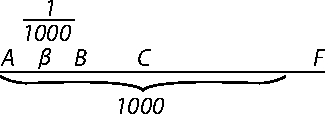
\includegraphics[width=0.24\textwidth]{gesamttex/edit_VIII,3/images/LH_35_09_15_001,022_d4.pdf}}%
%  \vspace*{0.5em}
%  \centerline{\hspace*{75mm}\lbrack\textit{Fig.~4}\rbrack}%
%  \vspace*{-0.5em}%
%
\pstart%
\footnotesize%
\noindent%
$BC \sqcap d\overline{s}$ \quad $AF \sqcap e$
% \protect\rule[0pt]{0mm}{20pt}%
\pend%
%
\pstart%
\vspace*{2.0em}%
\noindent%
\footnotesize%
$\displaystyle \frac{BC}{\frac{1}{1000}} \sqcap \frac{1999}{1000}$
\protect\rule[0pt]{0mm}{16pt}%
%
\newline%
$\displaystyle{BC \,\sqcap \frac{1999}{1000,000}} \,\sqcap\, d\overline{s}$
\protect\rule[0pt]{0mm}{16pt}
%
\newline%
$\displaystyle{AC \,\sqcap \frac{2999}{1000,000}} \,\sqcap s$
\protect\rule[0pt]{0mm}{16pt}%
%
\pend%
% \newpage%
%
% \newpage% Rein vorläufig !!!!
  \vspace*{-7.5em}%
  \centerline{\hspace*{45mm}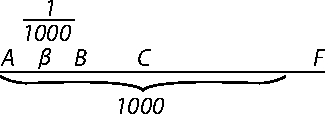
\includegraphics[width=0.24\textwidth]{gesamttex/edit_VIII,3/images/LH_35_09_15_001,022_d4.pdf}}%
  \vspace*{0.5em}
  \centerline{\hspace*{45mm}\lbrack\textit{Fig.~4}\rbrack}%
  \vspace*{-0.5em}%
  %
%  \vspace*{-6.0em}%
%  \centerline{\hspace*{45mm}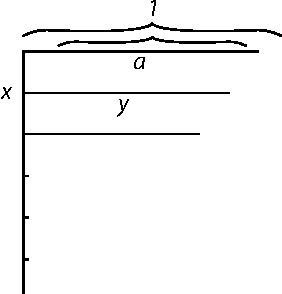
\includegraphics[width=0.22\textwidth]{gesamttex/edit_VIII,3/images/LH_35_09_15_001,022_d5.pdf}}%
%  \vspace*{-0.5em}
%  \centerline{\hspace*{45mm}\lbrack\textit{Fig.~5}\rbrack}%
%%  \newpage% Rein vorläufig !!!!
  \vspace*{4.5em}%
%
\pstart%
\footnotesize%
\noindent%
\edtext{$\beta \sqcap d\overline{x}$
\quad\quad%
$\displaystyle \frac{d\overline{s}}{\beta \sqcap d\overline{x}}$
}{%
\lemma{$\beta \sqcap d\overline{x}$}\Bfootnote{%
\textit{(1)}~$\displaystyle \frac{d\overline{s}}{\beta}$
\textit{(2)}~$\displaystyle \frac{d\overline{s}}{\beta \sqcap d\overline{x}}$%
~\textit{L}}}
aequ. $\frac{\textstyle{\!\int\!}\displaystyle{\overline{y \overline{x}}}}{\displaystyle{a}}$
\protect\rule[0pt]{0mm}{16pt}%
%
\newline%
$\displaystyle\frac{y}{a} \sqcap
\edtext{\frac{e - s}{e}$% 
\protect\rule[0pt]{0mm}{16pt}%
%
\newline%
Ergo}{%
\lemma{$\displaystyle \frac{e - s}{e}$}\Bfootnote{%
\textit{(1)}~$\displaystyle d\overline{z d\overline{z}} \,\sqcap$
\textit{(2)}~Ergo%
~\textit{L}}}
$\displaystyle d\overline{y} \sqcap
\edtext{-\frac{a}{e}d\overline{s}$%
\protect\rule[0pt]{0mm}{16pt}%
%
\newline%
Ergo}{%
\lemma{$\displaystyle-\frac{a}{e}d\overline{s}$}\Bfootnote{%
\textit{(1)}~$\displaystyle \frac{\cancel{z}\,d\overline{dz} + d}{\cancel{z}z}$
\textit{(2)}~Ergo%
~\textit{L}}}
$\displaystyle - \frac{e}{\cancel{a}} \frac{d\overline{y}}{dx} \sqcap \frac{\textstyle{\!\int\!}\displaystyle{\overline{y\,dx}}}{\cancel{a}}$
\edtext{et sit $y \sqcap zz$ fiet%
\protect\rule[0pt]{0mm}{16pt}}{%
\lemma{et}\Bfootnote{%
\textit{(1)}~$\displaystyle \frac{- b\,d\overline{d}y}{y} \sqcap d\overline{x}^2$
\textit{(2)}~$\displaystyle + \frac{d\overline{z} \,\efrac{\efrac{}{\leibvdash}}{}\, 2z\,dz}{z^4 - b zz}$ %
\textit{(3)}~sit $y \sqcap zz$ fiet $d\overline{dy}$
\textit{(4)}~sit $y \sqcap zz$ fiet %
~\textit{L}}}
{\normalsize{\lbrack\textit{\textit{Text bricht ab.}}\rbrack}}%
% $\pleibvdash$
%
\pend%
%
%
  \newpage% Rein vorläufig !!!!
  \pstart \vspace{1em} %\noindent
\begin{minipage}[t]{0.5\textwidth}
\hspace{11mm}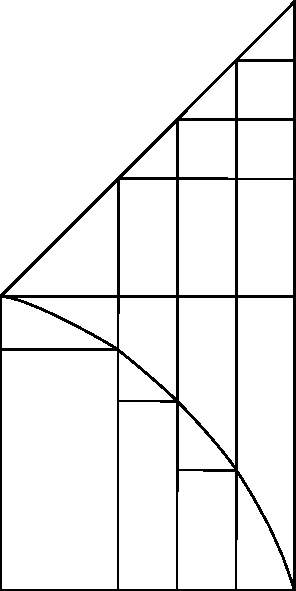
\includegraphics[width=0.37\textwidth]{gesamttex/edit_VIII,3/images/LH_35_09_15_001,022_d6.pdf}
\end{minipage}
\hspace{5mm}
\begin{minipage}[t]{0.5\textwidth}
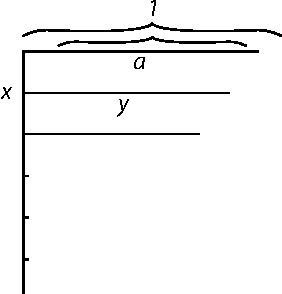
\includegraphics[width=0.5\textwidth]{gesamttex/edit_VIII,3/images/LH_35_09_15_001,022_d5.pdf}
\end{minipage}
%\vspace{3.5em}
\pend
\vspace{0.5em}
\pstart
 \hspace{16.5mm} [\textit{Fig.~5}]\hspace{55mm} [\textit{Fig.~6}]
\pend
\vspace{2em}

%  % \vspace*{0.0em}%
%  \centerline{\hspace{-45mm}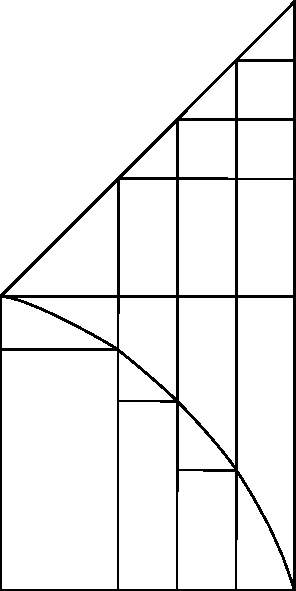
\includegraphics[width=0.16\textwidth]{gesamttex/edit_VIII,3/images/LH_35_09_15_001,022_d6.pdf}}%
%  \vspace{0.5em}
%  \centerline{\hspace{-45mm}\lbrack\textit{Fig.~5}\rbrack}%
%%  \newpage% Rein vorläufig !!!!
%%  \vspace*{1,0em}%
%  %
%  \vspace*{-10.0em}%
%  \centerline{\hspace{45mm}\hspace*{45mm}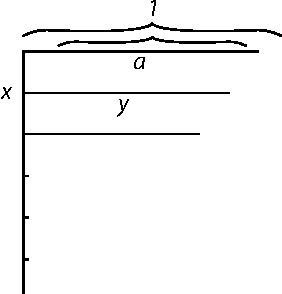
\includegraphics[width=0.22\textwidth]{gesamttex/edit_VIII,3/images/LH_35_09_15_001,022_d5.pdf}}%
%  \vspace*{-0.5em}
%  \centerline{\hspace{45mm}\hspace*{45mm}\lbrack\textit{Fig.~6}\rbrack}%
%%  \newpage% Rein vorläufig !!!!
%  \vspace*{4.0em}%
%%
%
\pstart%
\noindent%
\normalsize%
\lbrack\textit{Nebenrechnungen:}\rbrack\setline{1}%
\pend%
%
\vspace*{1.0em}%
\pstart%
\noindent%
\footnotesize%
\edtext{$1000000\\
\underline{\phantom{j00}2999}}{%
\lemma{1000000}\Bfootnote{%
\textit{(1)}~99997
\textit{(2)}~2999%
~\textit{L}}}\\
\setline{1}\phantom{0}997001$
\pend%
%
\vspace*{1.0em}%
\pstart%
\noindent%
\footnotesize%
$\phantom{000000}\underline{\phantom{g}999}\\
\phantom{000000}1000$\\
% \pend%
%
% \vspace*{1.0em}%
% \pstart%
% \noindent%
% \footnotesize%
\setline{1}$\underline{997001\phantom{gg}}\phantom{0}1\cdot2\\
\phantom{g}1000000$
\pend
\count\Bfootins=1200
\count\Afootins=1200
\count\Cfootins=1200%
%
% ENDE DES STÜCKES auf Blatt 22v 